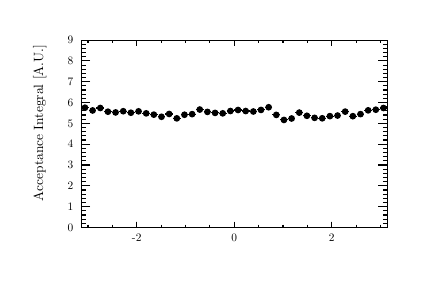
\begin{tikzpicture}
\pgfdeclareplotmark{cross} {
\pgfpathmoveto{\pgfpoint{-0.3\pgfplotmarksize}{\pgfplotmarksize}}
\pgfpathlineto{\pgfpoint{+0.3\pgfplotmarksize}{\pgfplotmarksize}}
\pgfpathlineto{\pgfpoint{+0.3\pgfplotmarksize}{0.3\pgfplotmarksize}}
\pgfpathlineto{\pgfpoint{+1\pgfplotmarksize}{0.3\pgfplotmarksize}}
\pgfpathlineto{\pgfpoint{+1\pgfplotmarksize}{-0.3\pgfplotmarksize}}
\pgfpathlineto{\pgfpoint{+0.3\pgfplotmarksize}{-0.3\pgfplotmarksize}}
\pgfpathlineto{\pgfpoint{+0.3\pgfplotmarksize}{-1.\pgfplotmarksize}}
\pgfpathlineto{\pgfpoint{-0.3\pgfplotmarksize}{-1.\pgfplotmarksize}}
\pgfpathlineto{\pgfpoint{-0.3\pgfplotmarksize}{-0.3\pgfplotmarksize}}
\pgfpathlineto{\pgfpoint{-1.\pgfplotmarksize}{-0.3\pgfplotmarksize}}
\pgfpathlineto{\pgfpoint{-1.\pgfplotmarksize}{0.3\pgfplotmarksize}}
\pgfpathlineto{\pgfpoint{-0.3\pgfplotmarksize}{0.3\pgfplotmarksize}}
\pgfpathclose
\pgfusepathqstroke
}
\pgfdeclareplotmark{cross*} {
\pgfpathmoveto{\pgfpoint{-0.3\pgfplotmarksize}{\pgfplotmarksize}}
\pgfpathlineto{\pgfpoint{+0.3\pgfplotmarksize}{\pgfplotmarksize}}
\pgfpathlineto{\pgfpoint{+0.3\pgfplotmarksize}{0.3\pgfplotmarksize}}
\pgfpathlineto{\pgfpoint{+1\pgfplotmarksize}{0.3\pgfplotmarksize}}
\pgfpathlineto{\pgfpoint{+1\pgfplotmarksize}{-0.3\pgfplotmarksize}}
\pgfpathlineto{\pgfpoint{+0.3\pgfplotmarksize}{-0.3\pgfplotmarksize}}
\pgfpathlineto{\pgfpoint{+0.3\pgfplotmarksize}{-1.\pgfplotmarksize}}
\pgfpathlineto{\pgfpoint{-0.3\pgfplotmarksize}{-1.\pgfplotmarksize}}
\pgfpathlineto{\pgfpoint{-0.3\pgfplotmarksize}{-0.3\pgfplotmarksize}}
\pgfpathlineto{\pgfpoint{-1.\pgfplotmarksize}{-0.3\pgfplotmarksize}}
\pgfpathlineto{\pgfpoint{-1.\pgfplotmarksize}{0.3\pgfplotmarksize}}
\pgfpathlineto{\pgfpoint{-0.3\pgfplotmarksize}{0.3\pgfplotmarksize}}
\pgfpathclose
\pgfusepathqfillstroke
}
\pgfdeclareplotmark{newstar} {
\pgfpathmoveto{\pgfqpoint{0pt}{\pgfplotmarksize}}
\pgfpathlineto{\pgfqpointpolar{44}{0.5\pgfplotmarksize}}
\pgfpathlineto{\pgfqpointpolar{18}{\pgfplotmarksize}}
\pgfpathlineto{\pgfqpointpolar{-20}{0.5\pgfplotmarksize}}
\pgfpathlineto{\pgfqpointpolar{-54}{\pgfplotmarksize}}
\pgfpathlineto{\pgfqpointpolar{-90}{0.5\pgfplotmarksize}}
\pgfpathlineto{\pgfqpointpolar{234}{\pgfplotmarksize}}
\pgfpathlineto{\pgfqpointpolar{198}{0.5\pgfplotmarksize}}
\pgfpathlineto{\pgfqpointpolar{162}{\pgfplotmarksize}}
\pgfpathlineto{\pgfqpointpolar{134}{0.5\pgfplotmarksize}}
\pgfpathclose
\pgfusepathqstroke
}
\pgfdeclareplotmark{newstar*} {
\pgfpathmoveto{\pgfqpoint{0pt}{\pgfplotmarksize}}
\pgfpathlineto{\pgfqpointpolar{44}{0.5\pgfplotmarksize}}
\pgfpathlineto{\pgfqpointpolar{18}{\pgfplotmarksize}}
\pgfpathlineto{\pgfqpointpolar{-20}{0.5\pgfplotmarksize}}
\pgfpathlineto{\pgfqpointpolar{-54}{\pgfplotmarksize}}
\pgfpathlineto{\pgfqpointpolar{-90}{0.5\pgfplotmarksize}}
\pgfpathlineto{\pgfqpointpolar{234}{\pgfplotmarksize}}
\pgfpathlineto{\pgfqpointpolar{198}{0.5\pgfplotmarksize}}
\pgfpathlineto{\pgfqpointpolar{162}{\pgfplotmarksize}}
\pgfpathlineto{\pgfqpointpolar{134}{0.5\pgfplotmarksize}}
\pgfpathclose
\pgfusepathqfillstroke
}
\definecolor{c}{rgb}{1,1,1};
\draw [color=c, fill=c] (0.1,0.0627517) rectangle (4.9,3.07483);
\draw [color=c, fill=c] (0.772,0.544685) rectangle (4.66,2.92423);
\definecolor{c}{rgb}{0,0,0};
\draw [c] (0.772,0.544685) -- (0.772,2.92423) -- (4.66,2.92423) -- (4.66,0.544685) -- (0.772,0.544685);
\draw [c,line width=0.4] (0.8206,2.03636) -- (0.8206,2.06591);
\draw [c,line width=0.4] (0.8206,2.06591) -- (0.8206,2.09545);
\draw [c,line width=0.4] (0.772,2.06591) -- (0.8206,2.06591);
\draw [c,line width=0.4] (0.8206,2.06591) -- (0.8692,2.06591);
\foreach \P in {(0.8206,2.06591)}{\draw[mark options={color=c,fill=c},mark size=2.402402pt,mark=*,mark size=1pt] plot coordinates {\P};}
\draw [c,line width=0.4] (0.9178,2.00134) -- (0.9178,2.03054);
\draw [c,line width=0.4] (0.9178,2.03054) -- (0.9178,2.05974);
\draw [c,line width=0.4] (0.8692,2.03054) -- (0.9178,2.03054);
\draw [c,line width=0.4] (0.9178,2.03054) -- (0.9664,2.03054);
\foreach \P in {(0.9178,2.03054)}{\draw[mark options={color=c,fill=c},mark size=2.402402pt,mark=*,mark size=1pt] plot coordinates {\P};}
\draw [c,line width=0.4] (1.015,2.03225) -- (1.015,2.06176);
\draw [c,line width=0.4] (1.015,2.06176) -- (1.015,2.09127);
\draw [c,line width=0.4] (0.9664,2.06176) -- (1.015,2.06176);
\draw [c,line width=0.4] (1.015,2.06176) -- (1.0636,2.06176);
\foreach \P in {(1.015,2.06176)}{\draw[mark options={color=c,fill=c},mark size=2.402402pt,mark=*,mark size=1pt] plot coordinates {\P};}
\draw [c,line width=0.4] (1.1122,1.98562) -- (1.1122,2.01466);
\draw [c,line width=0.4] (1.1122,2.01466) -- (1.1122,2.04371);
\draw [c,line width=0.4] (1.0636,2.01466) -- (1.1122,2.01466);
\draw [c,line width=0.4] (1.1122,2.01466) -- (1.1608,2.01466);
\foreach \P in {(1.1122,2.01466)}{\draw[mark options={color=c,fill=c},mark size=2.402402pt,mark=*,mark size=1pt] plot coordinates {\P};}
\draw [c,line width=0.4] (1.2094,1.97657) -- (1.2094,2.00552);
\draw [c,line width=0.4] (1.2094,2.00552) -- (1.2094,2.03448);
\draw [c,line width=0.4] (1.1608,2.00552) -- (1.2094,2.00552);
\draw [c,line width=0.4] (1.2094,2.00552) -- (1.258,2.00552);
\foreach \P in {(1.2094,2.00552)}{\draw[mark options={color=c,fill=c},mark size=2.402402pt,mark=*,mark size=1pt] plot coordinates {\P};}
\draw [c,line width=0.4] (1.3066,1.99186) -- (1.3066,2.02097);
\draw [c,line width=0.4] (1.3066,2.02097) -- (1.3066,2.05008);
\draw [c,line width=0.4] (1.258,2.02097) -- (1.3066,2.02097);
\draw [c,line width=0.4] (1.3066,2.02097) -- (1.3552,2.02097);
\foreach \P in {(1.3066,2.02097)}{\draw[mark options={color=c,fill=c},mark size=2.402402pt,mark=*,mark size=1pt] plot coordinates {\P};}
\draw [c,line width=0.4] (1.4038,1.97265) -- (1.4038,2.00156);
\draw [c,line width=0.4] (1.4038,2.00156) -- (1.4038,2.03048);
\draw [c,line width=0.4] (1.3552,2.00156) -- (1.4038,2.00156);
\draw [c,line width=0.4] (1.4038,2.00156) -- (1.4524,2.00156);
\foreach \P in {(1.4038,2.00156)}{\draw[mark options={color=c,fill=c},mark size=2.402402pt,mark=*,mark size=1pt] plot coordinates {\P};}
\draw [c,line width=0.4] (1.501,1.99018) -- (1.501,2.01927);
\draw [c,line width=0.4] (1.501,2.01927) -- (1.501,2.04836);
\draw [c,line width=0.4] (1.4524,2.01927) -- (1.501,2.01927);
\draw [c,line width=0.4] (1.501,2.01927) -- (1.5496,2.01927);
\foreach \P in {(1.501,2.01927)}{\draw[mark options={color=c,fill=c},mark size=2.402402pt,mark=*,mark size=1pt] plot coordinates {\P};}
\draw [c,line width=0.4] (1.5982,1.96487) -- (1.5982,1.99371);
\draw [c,line width=0.4] (1.5982,1.99371) -- (1.5982,2.02254);
\draw [c,line width=0.4] (1.5496,1.99371) -- (1.5982,1.99371);
\draw [c,line width=0.4] (1.5982,1.99371) -- (1.6468,1.99371);
\foreach \P in {(1.5982,1.99371)}{\draw[mark options={color=c,fill=c},mark size=2.402402pt,mark=*,mark size=1pt] plot coordinates {\P};}
\draw [c,line width=0.4] (1.6954,1.94869) -- (1.6954,1.97737);
\draw [c,line width=0.4] (1.6954,1.97737) -- (1.6954,2.00604);
\draw [c,line width=0.4] (1.6468,1.97737) -- (1.6954,1.97737);
\draw [c,line width=0.4] (1.6954,1.97737) -- (1.744,1.97737);
\foreach \P in {(1.6954,1.97737)}{\draw[mark options={color=c,fill=c},mark size=2.402402pt,mark=*,mark size=1pt] plot coordinates {\P};}
\draw [c,line width=0.4] (1.7926,1.92168) -- (1.7926,1.95008);
\draw [c,line width=0.4] (1.7926,1.95008) -- (1.7926,1.97848);
\draw [c,line width=0.4] (1.744,1.95008) -- (1.7926,1.95008);
\draw [c,line width=0.4] (1.7926,1.95008) -- (1.8412,1.95008);
\foreach \P in {(1.7926,1.95008)}{\draw[mark options={color=c,fill=c},mark size=2.402402pt,mark=*,mark size=1pt] plot coordinates {\P};}
\draw [c,line width=0.4] (1.8898,1.95726) -- (1.8898,1.98602);
\draw [c,line width=0.4] (1.8898,1.98602) -- (1.8898,2.01478);
\draw [c,line width=0.4] (1.8412,1.98602) -- (1.8898,1.98602);
\draw [c,line width=0.4] (1.8898,1.98602) -- (1.9384,1.98602);
\foreach \P in {(1.8898,1.98602)}{\draw[mark options={color=c,fill=c},mark size=2.402402pt,mark=*,mark size=1pt] plot coordinates {\P};}
\draw [c,line width=0.4] (1.987,1.90193) -- (1.987,1.93013);
\draw [c,line width=0.4] (1.987,1.93013) -- (1.987,1.95832);
\draw [c,line width=0.4] (1.9384,1.93013) -- (1.987,1.93013);
\draw [c,line width=0.4] (1.987,1.93013) -- (2.0356,1.93013);
\foreach \P in {(1.987,1.93013)}{\draw[mark options={color=c,fill=c},mark size=2.402402pt,mark=*,mark size=1pt] plot coordinates {\P};}
\draw [c,line width=0.4] (2.0842,1.94739) -- (2.0842,1.97605);
\draw [c,line width=0.4] (2.0842,1.97605) -- (2.0842,2.00471);
\draw [c,line width=0.4] (2.0356,1.97605) -- (2.0842,1.97605);
\draw [c,line width=0.4] (2.0842,1.97605) -- (2.1328,1.97605);
\foreach \P in {(2.0842,1.97605)}{\draw[mark options={color=c,fill=c},mark size=2.402402pt,mark=*,mark size=1pt] plot coordinates {\P};}
\draw [c,line width=0.4] (2.1814,1.95498) -- (2.1814,1.98371);
\draw [c,line width=0.4] (2.1814,1.98371) -- (2.1814,2.01245);
\draw [c,line width=0.4] (2.1328,1.98371) -- (2.1814,1.98371);
\draw [c,line width=0.4] (2.1814,1.98371) -- (2.23,1.98371);
\foreach \P in {(2.1814,1.98371)}{\draw[mark options={color=c,fill=c},mark size=2.402402pt,mark=*,mark size=1pt] plot coordinates {\P};}
\draw [c,line width=0.4] (2.2786,2.01279) -- (2.2786,2.0421);
\draw [c,line width=0.4] (2.2786,2.0421) -- (2.2786,2.07142);
\draw [c,line width=0.4] (2.23,2.0421) -- (2.2786,2.0421);
\draw [c,line width=0.4] (2.2786,2.0421) -- (2.3272,2.0421);
\foreach \P in {(2.2786,2.0421)}{\draw[mark options={color=c,fill=c},mark size=2.402402pt,mark=*,mark size=1pt] plot coordinates {\P};}
\draw [c,line width=0.4] (2.3758,1.98336) -- (2.3758,2.01238);
\draw [c,line width=0.4] (2.3758,2.01238) -- (2.3758,2.0414);
\draw [c,line width=0.4] (2.3272,2.01238) -- (2.3758,2.01238);
\draw [c,line width=0.4] (2.3758,2.01238) -- (2.4244,2.01238);
\foreach \P in {(2.3758,2.01238)}{\draw[mark options={color=c,fill=c},mark size=2.402402pt,mark=*,mark size=1pt] plot coordinates {\P};}
\draw [c,line width=0.4] (2.473,1.97066) -- (2.473,1.99956);
\draw [c,line width=0.4] (2.473,1.99956) -- (2.473,2.02845);
\draw [c,line width=0.4] (2.4244,1.99956) -- (2.473,1.99956);
\draw [c,line width=0.4] (2.473,1.99956) -- (2.5216,1.99956);
\foreach \P in {(2.473,1.99956)}{\draw[mark options={color=c,fill=c},mark size=2.402402pt,mark=*,mark size=1pt] plot coordinates {\P};}
\draw [c,line width=0.4] (2.5702,1.96511) -- (2.5702,1.99395);
\draw [c,line width=0.4] (2.5702,1.99395) -- (2.5702,2.02279);
\draw [c,line width=0.4] (2.5216,1.99395) -- (2.5702,1.99395);
\draw [c,line width=0.4] (2.5702,1.99395) -- (2.6188,1.99395);
\foreach \P in {(2.5702,1.99395)}{\draw[mark options={color=c,fill=c},mark size=2.402402pt,mark=*,mark size=1pt] plot coordinates {\P};}
\draw [c,line width=0.4] (2.6674,1.99431) -- (2.6674,2.02344);
\draw [c,line width=0.4] (2.6674,2.02344) -- (2.6674,2.05258);
\draw [c,line width=0.4] (2.6188,2.02344) -- (2.6674,2.02344);
\draw [c,line width=0.4] (2.6674,2.02344) -- (2.716,2.02344);
\foreach \P in {(2.6674,2.02344)}{\draw[mark options={color=c,fill=c},mark size=2.402402pt,mark=*,mark size=1pt] plot coordinates {\P};}
\draw [c,line width=0.4] (2.7646,2.00703) -- (2.7646,2.03629);
\draw [c,line width=0.4] (2.7646,2.03629) -- (2.7646,2.06554);
\draw [c,line width=0.4] (2.716,2.03629) -- (2.7646,2.03629);
\draw [c,line width=0.4] (2.7646,2.03629) -- (2.8132,2.03629);
\foreach \P in {(2.7646,2.03629)}{\draw[mark options={color=c,fill=c},mark size=2.402402pt,mark=*,mark size=1pt] plot coordinates {\P};}
\draw [c,line width=0.4] (2.8618,1.99411) -- (2.8618,2.02324);
\draw [c,line width=0.4] (2.8618,2.02324) -- (2.8618,2.05237);
\draw [c,line width=0.4] (2.8132,2.02324) -- (2.8618,2.02324);
\draw [c,line width=0.4] (2.8618,2.02324) -- (2.9104,2.02324);
\foreach \P in {(2.8618,2.02324)}{\draw[mark options={color=c,fill=c},mark size=2.402402pt,mark=*,mark size=1pt] plot coordinates {\P};}
\draw [c,line width=0.4] (2.959,1.98815) -- (2.959,2.01722);
\draw [c,line width=0.4] (2.959,2.01722) -- (2.959,2.04629);
\draw [c,line width=0.4] (2.9104,2.01722) -- (2.959,2.01722);
\draw [c,line width=0.4] (2.959,2.01722) -- (3.0076,2.01722);
\foreach \P in {(2.959,2.01722)}{\draw[mark options={color=c,fill=c},mark size=2.402402pt,mark=*,mark size=1pt] plot coordinates {\P};}
\draw [c,line width=0.4] (3.0562,2.0079) -- (3.0562,2.03716);
\draw [c,line width=0.4] (3.0562,2.03716) -- (3.0562,2.06643);
\draw [c,line width=0.4] (3.0076,2.03716) -- (3.0562,2.03716);
\draw [c,line width=0.4] (3.0562,2.03716) -- (3.1048,2.03716);
\foreach \P in {(3.0562,2.03716)}{\draw[mark options={color=c,fill=c},mark size=2.402402pt,mark=*,mark size=1pt] plot coordinates {\P};}
\draw [c,line width=0.4] (3.1534,2.04165) -- (3.1534,2.07125);
\draw [c,line width=0.4] (3.1534,2.07125) -- (3.1534,2.10085);
\draw [c,line width=0.4] (3.1048,2.07125) -- (3.1534,2.07125);
\draw [c,line width=0.4] (3.1534,2.07125) -- (3.202,2.07125);
\foreach \P in {(3.1534,2.07125)}{\draw[mark options={color=c,fill=c},mark size=2.402402pt,mark=*,mark size=1pt] plot coordinates {\P};}
\draw [c,line width=0.4] (3.2506,1.94565) -- (3.2506,1.97429);
\draw [c,line width=0.4] (3.2506,1.97429) -- (3.2506,2.00294);
\draw [c,line width=0.4] (3.202,1.97429) -- (3.2506,1.97429);
\draw [c,line width=0.4] (3.2506,1.97429) -- (3.2992,1.97429);
\foreach \P in {(3.2506,1.97429)}{\draw[mark options={color=c,fill=c},mark size=2.402402pt,mark=*,mark size=1pt] plot coordinates {\P};}
\draw [c,line width=0.4] (3.3478,1.88222) -- (3.3478,1.91022);
\draw [c,line width=0.4] (3.3478,1.91022) -- (3.3478,1.93821);
\draw [c,line width=0.4] (3.2992,1.91022) -- (3.3478,1.91022);
\draw [c,line width=0.4] (3.3478,1.91022) -- (3.3964,1.91022);
\foreach \P in {(3.3478,1.91022)}{\draw[mark options={color=c,fill=c},mark size=2.402402pt,mark=*,mark size=1pt] plot coordinates {\P};}
\draw [c,line width=0.4] (3.445,1.90023) -- (3.445,1.92841);
\draw [c,line width=0.4] (3.445,1.92841) -- (3.445,1.95659);
\draw [c,line width=0.4] (3.3964,1.92841) -- (3.445,1.92841);
\draw [c,line width=0.4] (3.445,1.92841) -- (3.4936,1.92841);
\foreach \P in {(3.445,1.92841)}{\draw[mark options={color=c,fill=c},mark size=2.402402pt,mark=*,mark size=1pt] plot coordinates {\P};}
\draw [c,line width=0.4] (3.5422,1.97428) -- (3.5422,2.00321);
\draw [c,line width=0.4] (3.5422,2.00321) -- (3.5422,2.03214);
\draw [c,line width=0.4] (3.4936,2.00321) -- (3.5422,2.00321);
\draw [c,line width=0.4] (3.5422,2.00321) -- (3.5908,2.00321);
\foreach \P in {(3.5422,2.00321)}{\draw[mark options={color=c,fill=c},mark size=2.402402pt,mark=*,mark size=1pt] plot coordinates {\P};}
\draw [c,line width=0.4] (3.6394,1.93423) -- (3.6394,1.96275);
\draw [c,line width=0.4] (3.6394,1.96275) -- (3.6394,1.99128);
\draw [c,line width=0.4] (3.5908,1.96275) -- (3.6394,1.96275);
\draw [c,line width=0.4] (3.6394,1.96275) -- (3.688,1.96275);
\foreach \P in {(3.6394,1.96275)}{\draw[mark options={color=c,fill=c},mark size=2.402402pt,mark=*,mark size=1pt] plot coordinates {\P};}
\draw [c,line width=0.4] (3.7366,1.90843) -- (3.7366,1.93669);
\draw [c,line width=0.4] (3.7366,1.93669) -- (3.7366,1.96496);
\draw [c,line width=0.4] (3.688,1.93669) -- (3.7366,1.93669);
\draw [c,line width=0.4] (3.7366,1.93669) -- (3.7852,1.93669);
\foreach \P in {(3.7366,1.93669)}{\draw[mark options={color=c,fill=c},mark size=2.402402pt,mark=*,mark size=1pt] plot coordinates {\P};}
\draw [c,line width=0.4] (3.8338,1.90278) -- (3.8338,1.93099);
\draw [c,line width=0.4] (3.8338,1.93099) -- (3.8338,1.9592);
\draw [c,line width=0.4] (3.7852,1.93099) -- (3.8338,1.93099);
\draw [c,line width=0.4] (3.8338,1.93099) -- (3.8824,1.93099);
\foreach \P in {(3.8338,1.93099)}{\draw[mark options={color=c,fill=c},mark size=2.402402pt,mark=*,mark size=1pt] plot coordinates {\P};}
\draw [c,line width=0.4] (3.931,1.9298) -- (3.931,1.95828);
\draw [c,line width=0.4] (3.931,1.95828) -- (3.931,1.98676);
\draw [c,line width=0.4] (3.8824,1.95828) -- (3.931,1.95828);
\draw [c,line width=0.4] (3.931,1.95828) -- (3.9796,1.95828);
\foreach \P in {(3.931,1.95828)}{\draw[mark options={color=c,fill=c},mark size=2.402402pt,mark=*,mark size=1pt] plot coordinates {\P};}
\draw [c,line width=0.4] (4.0282,1.9373) -- (4.0282,1.96586);
\draw [c,line width=0.4] (4.0282,1.96586) -- (4.0282,1.99441);
\draw [c,line width=0.4] (3.9796,1.96586) -- (4.0282,1.96586);
\draw [c,line width=0.4] (4.0282,1.96586) -- (4.0768,1.96586);
\foreach \P in {(4.0282,1.96586)}{\draw[mark options={color=c,fill=c},mark size=2.402402pt,mark=*,mark size=1pt] plot coordinates {\P};}
\draw [c,line width=0.4] (4.1254,1.98665) -- (4.1254,2.0157);
\draw [c,line width=0.4] (4.1254,2.0157) -- (4.1254,2.04476);
\draw [c,line width=0.4] (4.0768,2.0157) -- (4.1254,2.0157);
\draw [c,line width=0.4] (4.1254,2.0157) -- (4.174,2.0157);
\foreach \P in {(4.1254,2.0157)}{\draw[mark options={color=c,fill=c},mark size=2.402402pt,mark=*,mark size=1pt] plot coordinates {\P};}
\draw [c,line width=0.4] (4.2226,1.92943) -- (4.2226,1.95791);
\draw [c,line width=0.4] (4.2226,1.95791) -- (4.2226,1.98638);
\draw [c,line width=0.4] (4.174,1.95791) -- (4.2226,1.95791);
\draw [c,line width=0.4] (4.2226,1.95791) -- (4.2712,1.95791);
\foreach \P in {(4.2226,1.95791)}{\draw[mark options={color=c,fill=c},mark size=2.402402pt,mark=*,mark size=1pt] plot coordinates {\P};}
\draw [c,line width=0.4] (4.3198,1.95516) -- (4.3198,1.9839);
\draw [c,line width=0.4] (4.3198,1.9839) -- (4.3198,2.01264);
\draw [c,line width=0.4] (4.2712,1.9839) -- (4.3198,1.9839);
\draw [c,line width=0.4] (4.3198,1.9839) -- (4.3684,1.9839);
\foreach \P in {(4.3198,1.9839)}{\draw[mark options={color=c,fill=c},mark size=2.402402pt,mark=*,mark size=1pt] plot coordinates {\P};}
\draw [c,line width=0.4] (4.417,2.00274) -- (4.417,2.03195);
\draw [c,line width=0.4] (4.417,2.03195) -- (4.417,2.06117);
\draw [c,line width=0.4] (4.3684,2.03195) -- (4.417,2.03195);
\draw [c,line width=0.4] (4.417,2.03195) -- (4.4656,2.03195);
\foreach \P in {(4.417,2.03195)}{\draw[mark options={color=c,fill=c},mark size=2.402402pt,mark=*,mark size=1pt] plot coordinates {\P};}
\draw [c,line width=0.4] (4.5142,2.01071) -- (4.5142,2.04);
\draw [c,line width=0.4] (4.5142,2.04) -- (4.5142,2.0693);
\draw [c,line width=0.4] (4.4656,2.04) -- (4.5142,2.04);
\draw [c,line width=0.4] (4.5142,2.04) -- (4.5628,2.04);
\foreach \P in {(4.5142,2.04)}{\draw[mark options={color=c,fill=c},mark size=2.402402pt,mark=*,mark size=1pt] plot coordinates {\P};}
\draw [c,line width=0.4] (4.6114,2.03217) -- (4.6114,2.06168);
\draw [c,line width=0.4] (4.6114,2.06168) -- (4.6114,2.09118);
\draw [c,line width=0.4] (4.5628,2.06168) -- (4.6114,2.06168);
\draw [c,line width=0.4] (4.6114,2.06168) -- (4.66,2.06168);
\foreach \P in {(4.6114,2.06168)}{\draw[mark options={color=c,fill=c},mark size=2.402402pt,mark=*,mark size=1pt] plot coordinates {\P};}
\draw [c,line width=0.4] (0.772,0.544685) -- (4.66,0.544685);
\draw [anchor= east] (4.66,0.215042) node[scale=0.485847, rotate=0]{$\phihel$};
\draw [c,line width=0.4] (1.47778,0.617878) -- (1.47778,0.544685);
\draw [c,line width=0.4] (1.78734,0.581281) -- (1.78734,0.544685);
\draw [c,line width=0.4] (2.09689,0.581281) -- (2.09689,0.544685);
\draw [c,line width=0.4] (2.40645,0.581281) -- (2.40645,0.544685);
\draw [c,line width=0.4] (2.716,0.617878) -- (2.716,0.544685);
\draw [c,line width=0.4] (3.02555,0.581281) -- (3.02555,0.544685);
\draw [c,line width=0.4] (3.33511,0.581281) -- (3.33511,0.544685);
\draw [c,line width=0.4] (3.64466,0.581281) -- (3.64466,0.544685);
\draw [c,line width=0.4] (3.95422,0.617878) -- (3.95422,0.544685);
\draw [c,line width=0.4] (1.47778,0.617878) -- (1.47778,0.544685);
\draw [c,line width=0.4] (1.16823,0.581281) -- (1.16823,0.544685);
\draw [c,line width=0.4] (0.858675,0.581281) -- (0.858675,0.544685);
\draw [c,line width=0.4] (3.95422,0.617878) -- (3.95422,0.544685);
\draw [c,line width=0.4] (4.26377,0.581281) -- (4.26377,0.544685);
\draw [c,line width=0.4] (4.57332,0.581281) -- (4.57332,0.544685);
\draw [anchor=base] (1.47778,0.369984) node[scale=0.411101, rotate=0]{-2};
\draw [anchor=base] (2.716,0.369984) node[scale=0.411101, rotate=0]{0};
\draw [anchor=base] (3.95422,0.369984) node[scale=0.411101, rotate=0]{2};
\draw [c,line width=0.4] (0.772,2.92423) -- (4.66,2.92423);
\draw [c,line width=0.4] (1.47778,2.85103) -- (1.47778,2.92423);
\draw [c,line width=0.4] (1.78734,2.88763) -- (1.78734,2.92423);
\draw [c,line width=0.4] (2.09689,2.88763) -- (2.09689,2.92423);
\draw [c,line width=0.4] (2.40645,2.88763) -- (2.40645,2.92423);
\draw [c,line width=0.4] (2.716,2.85103) -- (2.716,2.92423);
\draw [c,line width=0.4] (3.02555,2.88763) -- (3.02555,2.92423);
\draw [c,line width=0.4] (3.33511,2.88763) -- (3.33511,2.92423);
\draw [c,line width=0.4] (3.64466,2.88763) -- (3.64466,2.92423);
\draw [c,line width=0.4] (3.95422,2.85103) -- (3.95422,2.92423);
\draw [c,line width=0.4] (1.47778,2.85103) -- (1.47778,2.92423);
\draw [c,line width=0.4] (1.16823,2.88763) -- (1.16823,2.92423);
\draw [c,line width=0.4] (0.858675,2.88763) -- (0.858675,2.92423);
\draw [c,line width=0.4] (3.95422,2.85103) -- (3.95422,2.92423);
\draw [c,line width=0.4] (4.26377,2.88763) -- (4.26377,2.92423);
\draw [c,line width=0.4] (4.57332,2.88763) -- (4.57332,2.92423);
\draw [c,line width=0.4] (0.772,0.544685) -- (0.772,2.92423);
\draw [anchor= east] (0.246688,2.92423) node[scale=0.485847, rotate=90]{Acceptance Integral [A.U.]};
\draw [c,line width=0.4] (0.88576,0.544685) -- (0.772,0.544685);
\draw [c,line width=0.4] (0.82888,0.597563) -- (0.772,0.597563);
\draw [c,line width=0.4] (0.82888,0.650442) -- (0.772,0.650442);
\draw [c,line width=0.4] (0.82888,0.703321) -- (0.772,0.703321);
\draw [c,line width=0.4] (0.82888,0.7562) -- (0.772,0.7562);
\draw [c,line width=0.4] (0.88576,0.809078) -- (0.772,0.809078);
\draw [c,line width=0.4] (0.82888,0.861957) -- (0.772,0.861957);
\draw [c,line width=0.4] (0.82888,0.914836) -- (0.772,0.914836);
\draw [c,line width=0.4] (0.82888,0.967715) -- (0.772,0.967715);
\draw [c,line width=0.4] (0.82888,1.02059) -- (0.772,1.02059);
\draw [c,line width=0.4] (0.88576,1.07347) -- (0.772,1.07347);
\draw [c,line width=0.4] (0.82888,1.12635) -- (0.772,1.12635);
\draw [c,line width=0.4] (0.82888,1.17923) -- (0.772,1.17923);
\draw [c,line width=0.4] (0.82888,1.23211) -- (0.772,1.23211);
\draw [c,line width=0.4] (0.82888,1.28499) -- (0.772,1.28499);
\draw [c,line width=0.4] (0.88576,1.33787) -- (0.772,1.33787);
\draw [c,line width=0.4] (0.82888,1.39074) -- (0.772,1.39074);
\draw [c,line width=0.4] (0.82888,1.44362) -- (0.772,1.44362);
\draw [c,line width=0.4] (0.82888,1.4965) -- (0.772,1.4965);
\draw [c,line width=0.4] (0.82888,1.54938) -- (0.772,1.54938);
\draw [c,line width=0.4] (0.88576,1.60226) -- (0.772,1.60226);
\draw [c,line width=0.4] (0.82888,1.65514) -- (0.772,1.65514);
\draw [c,line width=0.4] (0.82888,1.70802) -- (0.772,1.70802);
\draw [c,line width=0.4] (0.82888,1.7609) -- (0.772,1.7609);
\draw [c,line width=0.4] (0.82888,1.81377) -- (0.772,1.81377);
\draw [c,line width=0.4] (0.88576,1.86665) -- (0.772,1.86665);
\draw [c,line width=0.4] (0.82888,1.91953) -- (0.772,1.91953);
\draw [c,line width=0.4] (0.82888,1.97241) -- (0.772,1.97241);
\draw [c,line width=0.4] (0.82888,2.02529) -- (0.772,2.02529);
\draw [c,line width=0.4] (0.82888,2.07817) -- (0.772,2.07817);
\draw [c,line width=0.4] (0.88576,2.13105) -- (0.772,2.13105);
\draw [c,line width=0.4] (0.82888,2.18393) -- (0.772,2.18393);
\draw [c,line width=0.4] (0.82888,2.2368) -- (0.772,2.2368);
\draw [c,line width=0.4] (0.82888,2.28968) -- (0.772,2.28968);
\draw [c,line width=0.4] (0.82888,2.34256) -- (0.772,2.34256);
\draw [c,line width=0.4] (0.88576,2.39544) -- (0.772,2.39544);
\draw [c,line width=0.4] (0.82888,2.44832) -- (0.772,2.44832);
\draw [c,line width=0.4] (0.82888,2.5012) -- (0.772,2.5012);
\draw [c,line width=0.4] (0.82888,2.55408) -- (0.772,2.55408);
\draw [c,line width=0.4] (0.82888,2.60696) -- (0.772,2.60696);
\draw [c,line width=0.4] (0.88576,2.65983) -- (0.772,2.65983);
\draw [c,line width=0.4] (0.82888,2.71271) -- (0.772,2.71271);
\draw [c,line width=0.4] (0.82888,2.76559) -- (0.772,2.76559);
\draw [c,line width=0.4] (0.82888,2.81847) -- (0.772,2.81847);
\draw [c,line width=0.4] (0.82888,2.87135) -- (0.772,2.87135);
\draw [c,line width=0.4] (0.88576,2.92423) -- (0.772,2.92423);
\draw [anchor= east] (0.724,0.544685) node[scale=0.411101, rotate=0]{0};
\draw [anchor= east] (0.724,0.809078) node[scale=0.411101, rotate=0]{1};
\draw [anchor= east] (0.724,1.07347) node[scale=0.411101, rotate=0]{2};
\draw [anchor= east] (0.724,1.33787) node[scale=0.411101, rotate=0]{3};
\draw [anchor= east] (0.724,1.60226) node[scale=0.411101, rotate=0]{4};
\draw [anchor= east] (0.724,1.86665) node[scale=0.411101, rotate=0]{5};
\draw [anchor= east] (0.724,2.13105) node[scale=0.411101, rotate=0]{6};
\draw [anchor= east] (0.724,2.39544) node[scale=0.411101, rotate=0]{7};
\draw [anchor= east] (0.724,2.65983) node[scale=0.411101, rotate=0]{8};
\draw [anchor= east] (0.724,2.92423) node[scale=0.411101, rotate=0]{9};
\draw [c,line width=0.4] (4.66,0.544685) -- (4.66,2.92423);
\draw [c,line width=0.4] (4.54624,0.544685) -- (4.66,0.544685);
\draw [c,line width=0.4] (4.60312,0.597563) -- (4.66,0.597563);
\draw [c,line width=0.4] (4.60312,0.650442) -- (4.66,0.650442);
\draw [c,line width=0.4] (4.60312,0.703321) -- (4.66,0.703321);
\draw [c,line width=0.4] (4.60312,0.7562) -- (4.66,0.7562);
\draw [c,line width=0.4] (4.54624,0.809078) -- (4.66,0.809078);
\draw [c,line width=0.4] (4.60312,0.861957) -- (4.66,0.861957);
\draw [c,line width=0.4] (4.60312,0.914836) -- (4.66,0.914836);
\draw [c,line width=0.4] (4.60312,0.967715) -- (4.66,0.967715);
\draw [c,line width=0.4] (4.60312,1.02059) -- (4.66,1.02059);
\draw [c,line width=0.4] (4.54624,1.07347) -- (4.66,1.07347);
\draw [c,line width=0.4] (4.60312,1.12635) -- (4.66,1.12635);
\draw [c,line width=0.4] (4.60312,1.17923) -- (4.66,1.17923);
\draw [c,line width=0.4] (4.60312,1.23211) -- (4.66,1.23211);
\draw [c,line width=0.4] (4.60312,1.28499) -- (4.66,1.28499);
\draw [c,line width=0.4] (4.54624,1.33787) -- (4.66,1.33787);
\draw [c,line width=0.4] (4.60312,1.39074) -- (4.66,1.39074);
\draw [c,line width=0.4] (4.60312,1.44362) -- (4.66,1.44362);
\draw [c,line width=0.4] (4.60312,1.4965) -- (4.66,1.4965);
\draw [c,line width=0.4] (4.60312,1.54938) -- (4.66,1.54938);
\draw [c,line width=0.4] (4.54624,1.60226) -- (4.66,1.60226);
\draw [c,line width=0.4] (4.60312,1.65514) -- (4.66,1.65514);
\draw [c,line width=0.4] (4.60312,1.70802) -- (4.66,1.70802);
\draw [c,line width=0.4] (4.60312,1.7609) -- (4.66,1.7609);
\draw [c,line width=0.4] (4.60312,1.81377) -- (4.66,1.81377);
\draw [c,line width=0.4] (4.54624,1.86665) -- (4.66,1.86665);
\draw [c,line width=0.4] (4.60312,1.91953) -- (4.66,1.91953);
\draw [c,line width=0.4] (4.60312,1.97241) -- (4.66,1.97241);
\draw [c,line width=0.4] (4.60312,2.02529) -- (4.66,2.02529);
\draw [c,line width=0.4] (4.60312,2.07817) -- (4.66,2.07817);
\draw [c,line width=0.4] (4.54624,2.13105) -- (4.66,2.13105);
\draw [c,line width=0.4] (4.60312,2.18393) -- (4.66,2.18393);
\draw [c,line width=0.4] (4.60312,2.2368) -- (4.66,2.2368);
\draw [c,line width=0.4] (4.60312,2.28968) -- (4.66,2.28968);
\draw [c,line width=0.4] (4.60312,2.34256) -- (4.66,2.34256);
\draw [c,line width=0.4] (4.54624,2.39544) -- (4.66,2.39544);
\draw [c,line width=0.4] (4.60312,2.44832) -- (4.66,2.44832);
\draw [c,line width=0.4] (4.60312,2.5012) -- (4.66,2.5012);
\draw [c,line width=0.4] (4.60312,2.55408) -- (4.66,2.55408);
\draw [c,line width=0.4] (4.60312,2.60696) -- (4.66,2.60696);
\draw [c,line width=0.4] (4.54624,2.65983) -- (4.66,2.65983);
\draw [c,line width=0.4] (4.60312,2.71271) -- (4.66,2.71271);
\draw [c,line width=0.4] (4.60312,2.76559) -- (4.66,2.76559);
\draw [c,line width=0.4] (4.60312,2.81847) -- (4.66,2.81847);
\draw [c,line width=0.4] (4.60312,2.87135) -- (4.66,2.87135);
\draw [c,line width=0.4] (4.54624,2.92423) -- (4.66,2.92423);
\end{tikzpicture}
